% !TeX root = ../../../main.tex


\begin{figure}
	\centering
	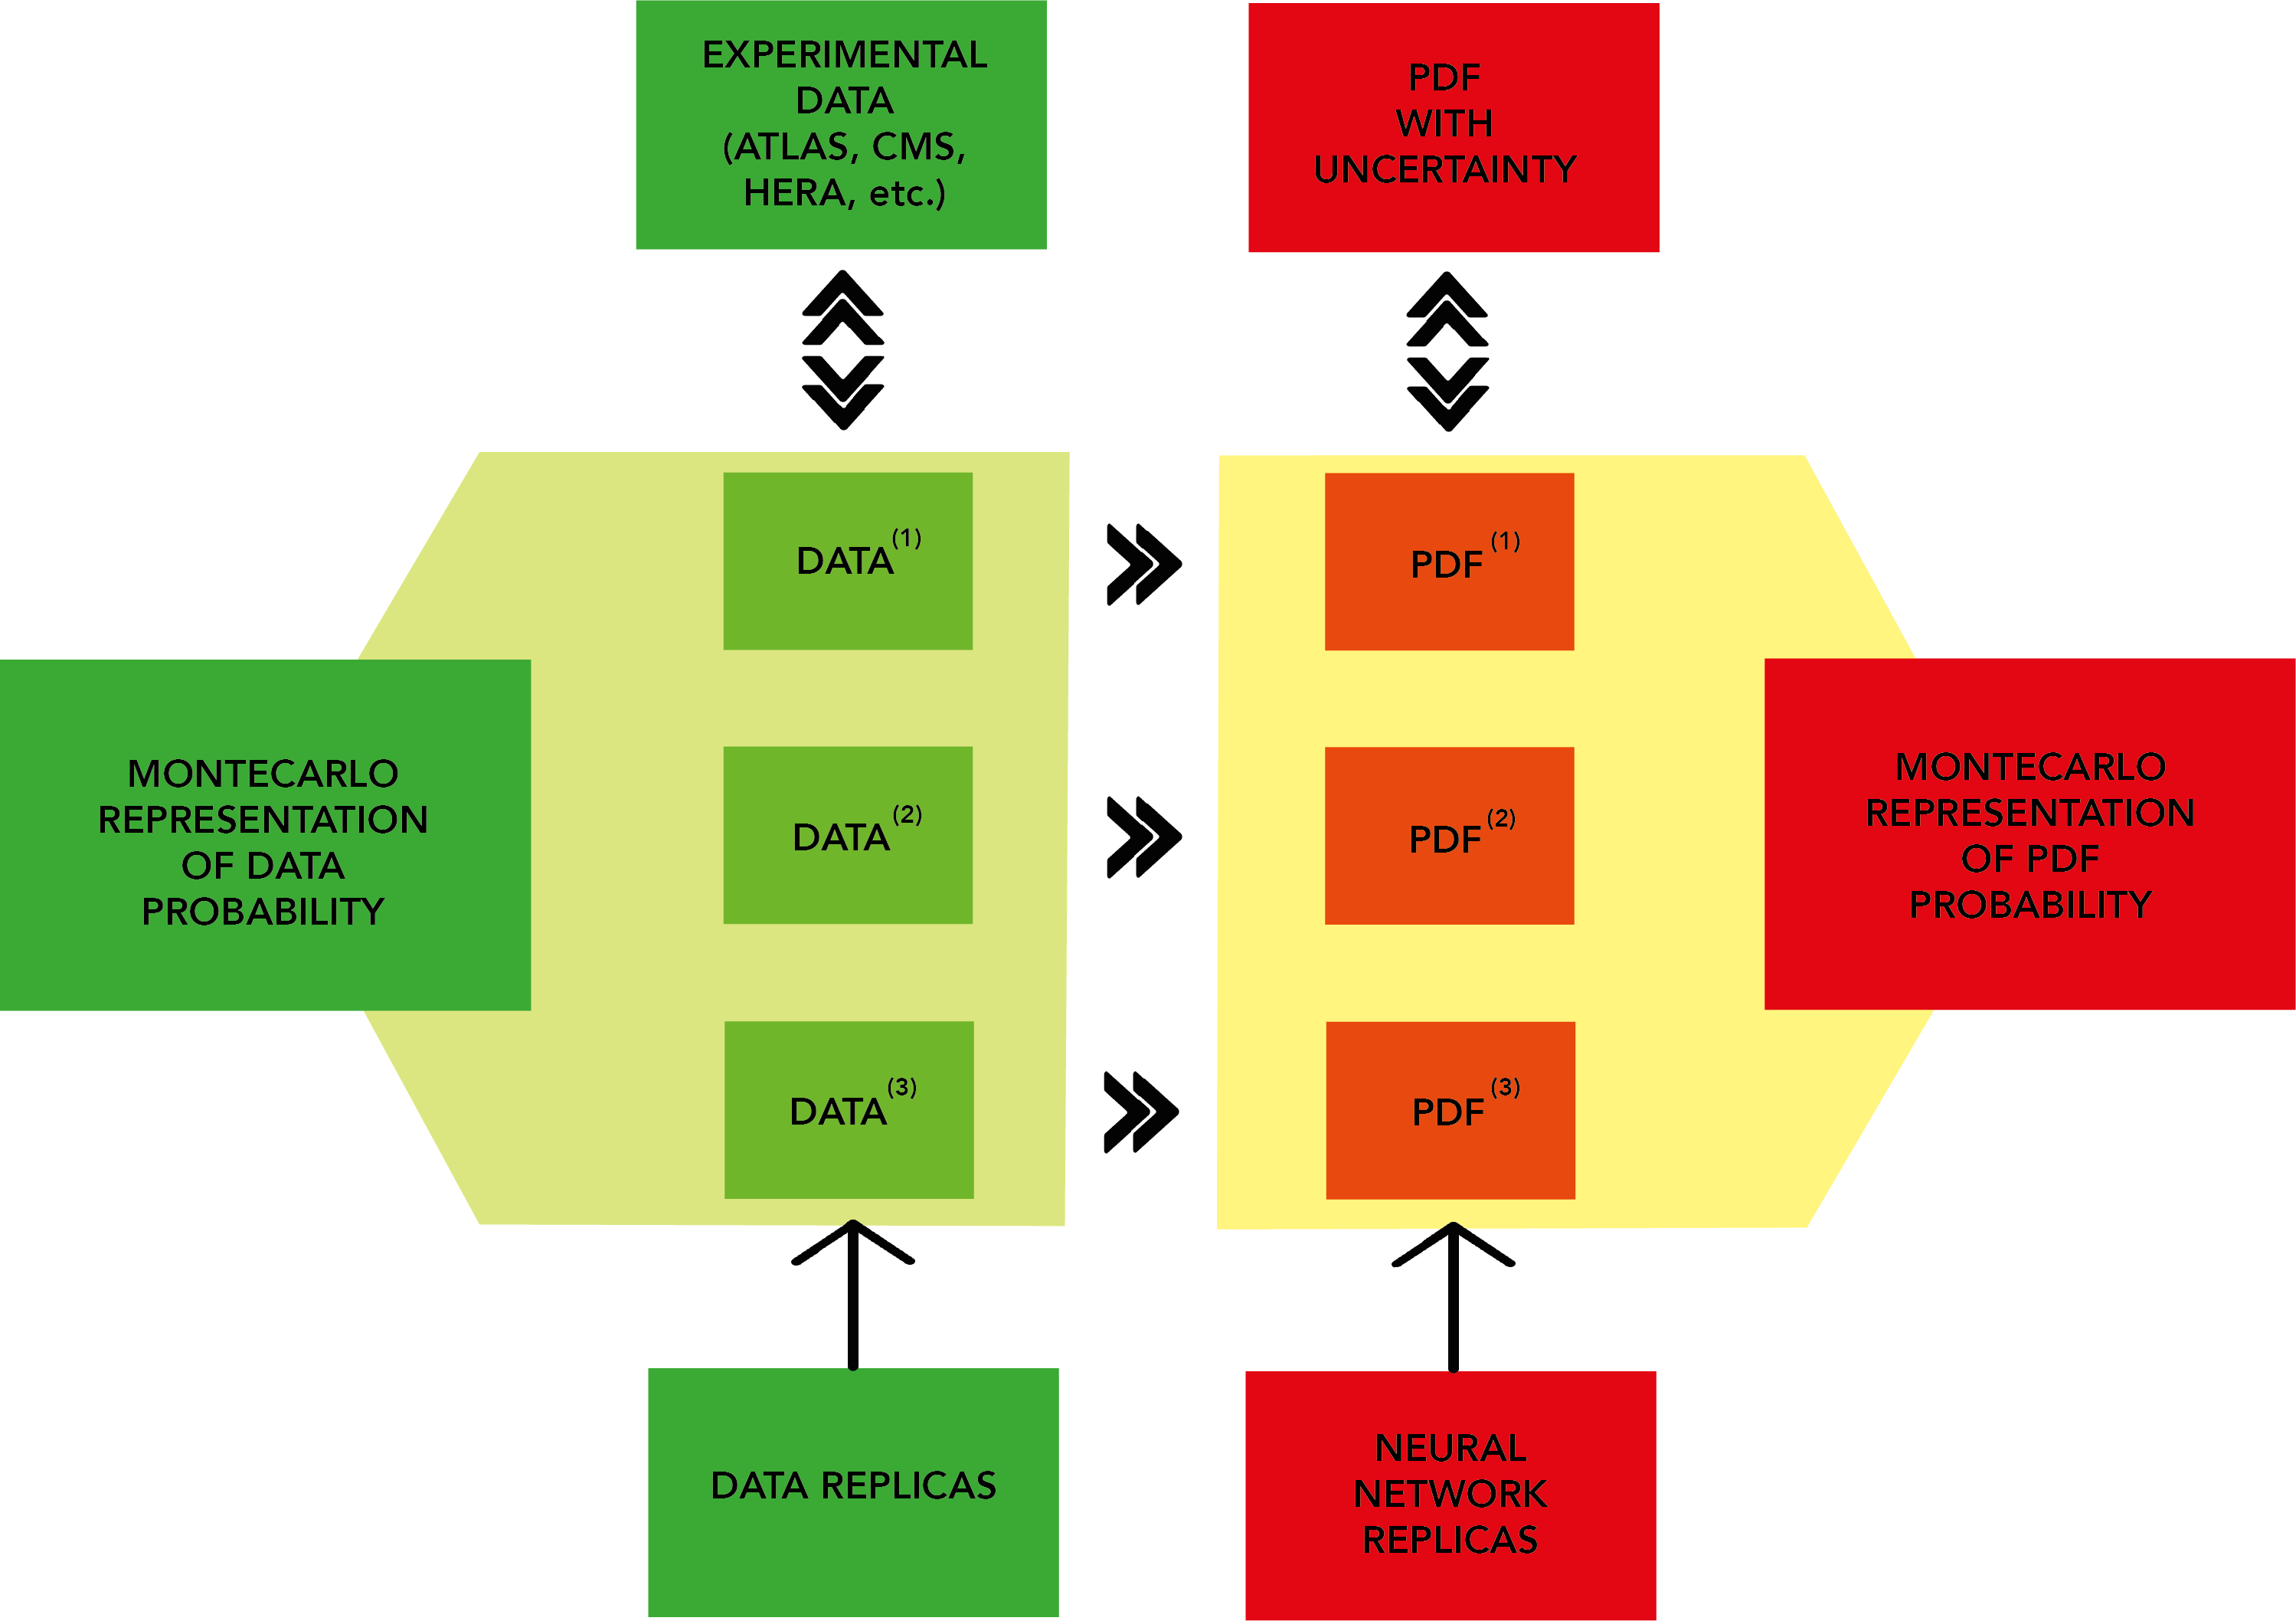
\includegraphics[width=\hsize]{ch-gp/nnpdf-strategy}
	\caption{
    \nnpdf uncertainty propagation methodology, one of the most important key
    points of \nnpdf methodology.
    Picture available on the collaboration website
    \url{http://nnpdf.mi.infn.it/research/general-strategy/}.
	}
	\label{fig:gp/nnpdf}
\end{figure}

- validating assumptions: closure tests
  - brief mention to inconsistent data
  - i.e. CT act as if finite order theory were exact, and data as well

\subsection{Generalization}

- tr/vl split
- hyperopt
- future tests
- larger error in extrap region: mention afb

\subsection{Minor improvements}

- sampling with negative values
- fast thcovmat construction
